\section{HARDWARE PLATFORM}
\subsection{Structure of Link Module}
We constructed the link module of the multilinks as shown in \figref{hardware}(a). Each link module has a build-in propeller at the center and a servo motor at the end of the link module comprised the main part of the joint module. The rotation range of each joint is $-\frac{\pi}{2}$[rad] $\sim \frac{\pi}{2}$[rad]. The multilinks can transform only in two-dimensions due to the joints with the same rotational axis. The range of lifting force is (0[N]$\sim$16.5[N]). The length of each link is 0.6[m] while the diameter of the propeller protector is 0.38[m]. The main square pipe is made of carbon.

\begin{figure}[t]
  \begin{center}
    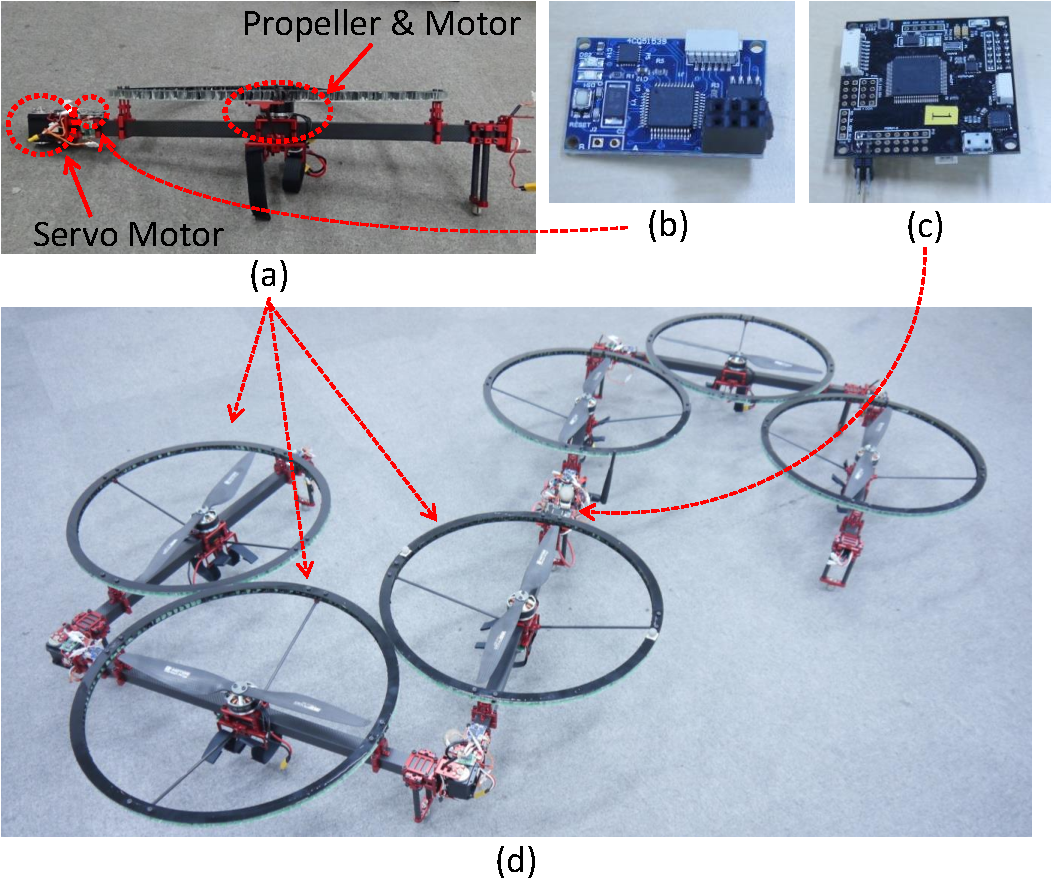
\includegraphics[width=1.0\columnwidth]{figs/hardware.pdf}
  \end{center}
  \caption{The hardware components of the multilinked multirotor. (a): the link module of multilinks with built-in propeller at the center, servo motor at the end and controller board(Neuron). (b): controller board Neuron communicating with each device and comprising IMU onboard. (c): controller board Spinal communicating with each Neuron and the onboard computer. (d): transformable hex-rotor with six-links consisting of the link modules. \label{figure:hardware}}
\end{figure}

\subsection{Multi-drop Structure for Internal Communication}
The multirotor with multilinks has not only motors for rotation of propeller but also servo motors for transform as actuator. Besides, the length of the multilinks is longer than conventional aerial robots. In our previous work\cite{Zhao2016}, the multilinks has only one central processor connected to all actuators and sensors. However, it is assumed that if we provide the conventional method for the multilinks, the possibility of disconnection increases due to the length of the multilinks. Matsui et al.\cite{Matsui2005} made reference to this problem for humanoid robots. Moreover, changing the number of links is difficult.
\par
For the reason noted above, we constructed multi-drop structure for internal communication(\figref{internal_communication}). As shown in \figref{hardware}(a), each link module has the controller board(Neuron)(\figref{hardware}(b)) which sends data to the motor and the servo motor and receives data from IMU(Inertia Measurement Unit). Moreover, the center link has the other controller board(Spinal)(\figref{hardware}(c)) which communicates with each Neuron. We use CAN(Controller Area Network)\cite{CAN} to construct the communication system between the controller boards. As used in cars, CAN is a reliable communication system which resists external noise. Each Neuron has an ID for identification of data. The onboard computer is connected to Spinal on USB-serial communication. The LQI control, motion planning, etc. are executed on the computer. 
\par
Through the main pipe, only two cables which are a power cable and a CAN cable are passed. Thereby, the amount of electric wiring decreases resulting that the high reliability of the communication improves. In addition, changing the number of links becomes easier. To add a link, we must just connect the two cables and configure the ID of Neuron. 

\begin{figure}[t]
  \begin{center}
    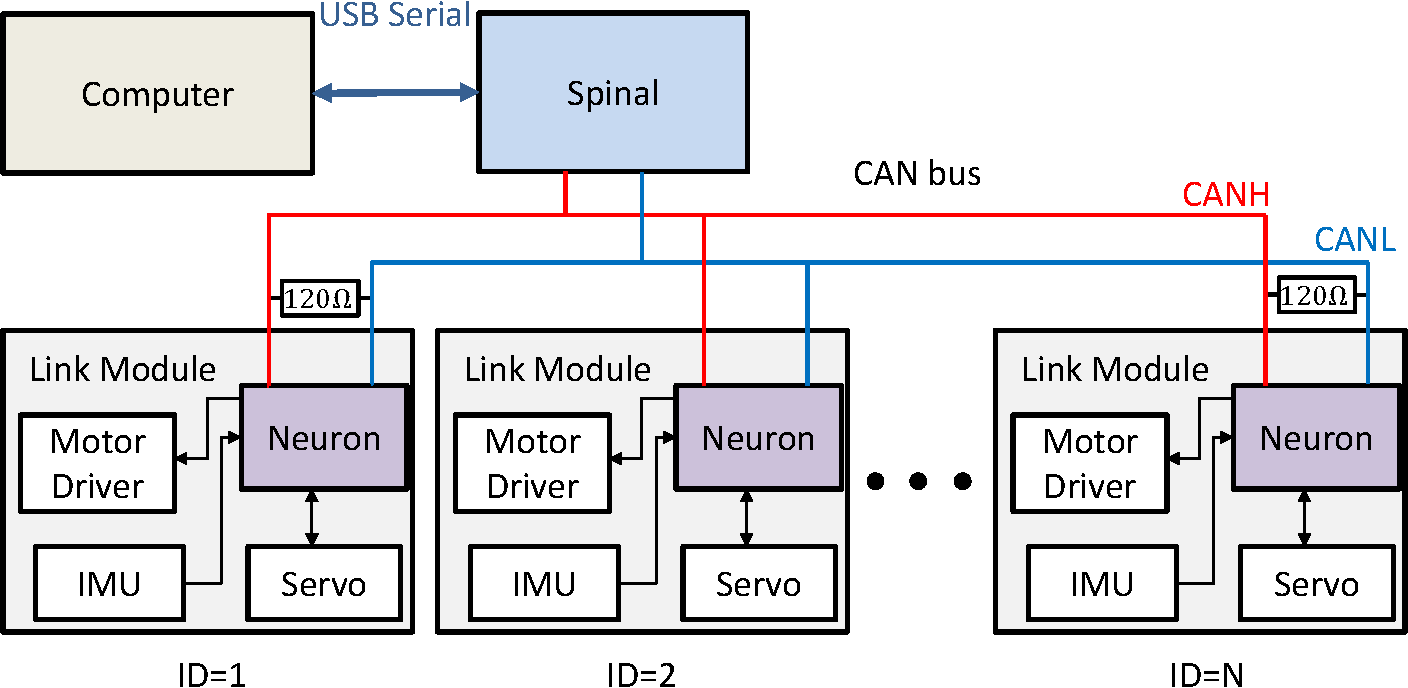
\includegraphics[width=1.0\columnwidth]{figs/internal_communication.pdf}
  \end{center}
  \caption{The multi-drop structure for internal communication comprising Neuron, Spinal and Computer: Neuron communicates with each device(motor, servo motor and IMU) while Spinal communicates with Neuron by using CAN. Computer and Spinal communicate by using USB-Serial.\label{figure:internal_communication}}
\end{figure}
